% !TeX root = RJwrapper.tex
\title{QTLEMM: An R Package for QTL Mapping and Hotspot Detection}
\author{by Ping-Yuan Chung, You-Tsz Guo, Hsiang-An Ho, Hsin-I Lee, Po-Ya Wu, Man-Hsia Yang,	Miao-Hui Zeng, and Chen-Hung Kao}

\maketitle


\abstract{This paper introduces an R package QTLEMM that implements commonly used and popular statistical methods for QTL mapping and QTL hotspot detection. For QTL mapping, QTLEMM offers a suite of functions for simulating data, computing significance thresholds, and estimating QTL parameters using single-QTL or multiple-QTL methods in diverse experimental populations. These methods encompass linear regression, permutation tests, Gaussian stochastic process, normal mixture models, and truncated normal mixture models. Moreover, QTLEMM accommodates both complete genotyping and selective genotyping data, and enables the fitting and comparison of different models in the analysis. For QTL hotspot detection, QTLEMM devises the statistical framework that can handle both the data from genetical genomics experiments and summarized data, mitigate the underestimation of hotspot thresholds, and also identify various types of hotspots at a very low computational cost. QTLEMM provides numerical and graphical results, and can facilitate the discovery of more significant results in the analysis of quantitative traits in biological studies.}

\section{Introduction}

Many biologically and economically important traits in organisms are quantitative rather than qualitative. These include traditional traits (such as yields and quality in rice, weight and body fat percentage in animals, and diabetes and hypertension in humans) and molecular traits (such as gene expression and protein levels). Quantitative traits typically exhibit continuous variation in a population, so there is no easy way to categorize them. They are likely to be affected by numerous genes each with modest effects and easily affected by environmental factors \citep{Falconer-1996}. Consequently, traditional methods such as the Mendelian segregation ratio analysis, mean and variance analyses, covariance studies, and the examination of familial correlations are very difficult for detecting the individual genes contributing to these traits. The genes responsible for quantitative traits are referred to as quantitative trait loci (QTL). For a long time, researchers have tried to obtain individual QTL information for exploring the genetic mechanisms underlying quantitative traits and further to manipulate them for improving the traits. With the availability of fine-scale genetic marker data along the genomes for various organisms, it has become possible to systematically map for and detect individual QTL (QTL mapping) by using more sophisticated statistical methods. Understanding the genetic mechanisms of quantitative traits using QTL mapping remains a major challenge and considerable issue in broad areas of biological studies \citep{Chen-2020, Kumar-2024, Meng-2024, Mackay-2024}. 

Statistical methods for QTL mapping have been well established \citep{Lander-1989, Haley-1992, Zeng-1993, Jansen-1993, Zeng-1994, Xu-1995, Kao-1999, Kao-2000, Sen-2001, Broman-2003, Kao-2002, Kao-2004, Kao-2006, Verbyla-2007, Li-2008, Kao-2009, Kao-2010, Kao-2012, Lee-2014, Wang-2016}. These methods analyze the marker and trait data from well-designed experimental populations to estimate the QTL parameters,  including the numbers, positions, various gene effects (additive, dominance, and interactive), variance components, heritabilities, etc. The experimental populations include the most commonly used populations, such as the backcross and $F_2$ populations, and other more advanced populations, such as recombinant inbred (RI) populations, advanced intercross (AI) populations, intermated recombinant inbred (IRI) populations, and immortalized $F_2$ populations \citep{Kao-2009}. The statistical methods are applied to analyze the QTL mapping data and tackle several central issues, including the estimation of QTL parameters, determination of threshold values and selective genotyping, in the QTL mapping studies. These studies have provided important insights into the genetic mechanisms governing quantitative traits in various organisms, such as rice, maize, alfalfa, Atlantic salmon, trout, etc. \citep{Vaughan-2007, Chen-2020, Kumar-2024, Meng-2024, Mackay-2024}.

QTL hotspots, characterized by genomic locations enriched in QTL, represent a common and notable feature when collecting numerous QTL for various traits in various biological studies \citep{Chardon-2004, West-2007, Breitling-2008, Wu-2008, Yang-2019, Meng-2024}. These hotspots are significant and appealing due to their high informativeness and potential harboring for genes related to quantitative traits. Presently, both the data containing original marker genotypes and numerous molecular traits for each individual (referred to as individual-level data hereafter) from genetical genomics experiments and the summarized QTL data from public QTL databases can provide the data sets with numerous QTL for hotspot analysis. Statistical methods using either type of data for detecting QTL hotspots have been proposed, and they are mainly based on the permutation test approach \citep{Wu-2008, Li-2010, Breitling-2008, Neto-2012, Yang-2019, Wu-2021}. Among these methods, the statistical framework outlined by \citet{Yang-2019} and \citet{Wu-2021} has the notable features of being able to handle both types of data, addresses several challenges and saves computational cost in the process of QTL hotspot detection.

Statistical QTL mapping software packages such as MapMaker/QTL \citep{Lincoln-1993}, WinQTLCart \citep{Wang-2000}, R/\CRANpkg{qtl} \citep{Broman-2003}, QTLNetwork \citep{Yang-2008, Taylor-2011, Verbyla-2012}, QTL.gCIMapping.GUI \citep{Zhang-2020} have been developed and documented in the literature. Among them, while most packages consider fixed effect models, the R/\CRANpkg{wgaim} package developed in the R system offers linear mixed effects and random effects models, respectively, for QTL mapping in the backcross, DH and RIL populations. It has the feature of being able to simultaneously incorporate the whole genome into the model, and hence is relatively simple in selecting and detecting QTL during the analysis \citep{Taylor-2011}. Notably, R/\CRANpkg{qtl} is a free and powerful R package that provides a broad range of methods, which include single-marker analysis, interval mapping \citep{Lander-1989}, regression interval mapping \citep{Haley-1992}, multiple QTL mapping \citep{Jansen-1993},  composite interval mapping \citep{Zeng-1994} for a wide variety of experimental populations for QTL mapping. Permutation test \citep{Churchill-1994} is used to determine significance thresholds for QTL mapping in R/\CRANpkg{qtl}. Here, we introduce an R package \CRANpkg{QTLEMM} (QTL EM algorithm mapping) that implements commonly used and popular statistical methods for both QTL mapping and QTL hotspot detection. For QTL mapping analysis, in addition to providing most of the methods in R/\CRANpkg{qtl}, \CRANpkg{QTLEMM}  also offers multiple interval mapping \citep{Kao-1999} to fit multiple QTL directly in the model for a wide range of experimental populations. Furthermore, \CRANpkg{QTLEMM} can perform novel tasks that the existing R packages lack such as simulating and handling the complete or selective genotyping data, computing the significance threshold values based on Gaussian stochastic process, and providing the asymptotic variance-covariance matrix for the QTL estimates \citep{Kao-1997, Kao-2012, Lee-2014}. \CRANpkg{QTLEMM} also distinguishes itself by uniquely offering the statistical framework of \citet{Yang-2019} and \citet{Wu-2021} using either the individual-level data or summarized data to proceed with the QTL hotspot detection analysis. We provide a comprehensive overview of the primary R functions in the \CRANpkg{QTLEMM} package. Results from analyses are presented through numerical and graphical outputs, facilitating interpretation and visualization of findings. The \CRANpkg{QTLEMM} package provides researchers with statistical tools to find more significant results in exploring the network among expression of genes, QTL hotspots, and quantitative traits in genes, genomes, and genetics studies.

\section{Statistical methods}

Identifying individual QTL (QTL mapping) is a crucial endeavor aimed at understanding the genetic basis and architecture of quantitative traits, thereby facilitating trait manipulation and improvement. Since the specific locations of QTLs are unknown prior to mapping and they could potentially be located anywhere along the genome, the primary objectives of statistical methods are centered around searching for individual QTLs and subsequently fitting them all into statistical model for the estimation of QTL parameters.

\subsection{QTL mapping models}

\citet{Lander-1989} were the first to propose a QTL mapping procedure known as interval mapping, which systematically searches the entire genome for QTLs. The interval mapping approach utilizes one marker interval (one flanking marker pair) at a time to establish a putative QTL at a specific position. It models the relationship between a quantitative trait and the putative QTL at that position, subsequently testing for the presence of the QTL. For a putative QTL, denoted as Q, at a specific fixed position x along the genome, the statistical model for individual $i$ with a phenotypic trait value $y_{i}$ can be expressed as follows: 

\begin{equation} 
	y_{i} = G_{i} + \varepsilon_{i} \label{eq:e1}
\end{equation} 

\noindent where $G_{i}$ represents the genotypic value of individual $i$, and $\varepsilon_{i}$ is a residual assumed to follow a normal distribution with mean $0$ and variance $\sigma ^{2}$. For the individuals in a population derived from two inbred lines, such as the $F_2$ population, the genotypes of their Q can be one of the three possible genotypes, $P_{1}$ homozygote ($QQ$), heterozygote ($Qq$) or $P_{2}$ homozygote ($qq$). Several different genetic models have been proposed to characterize the relationship between genotypic values and gene effects \citep{Cockerham-1954, van-1959, Weir-1977, Kao-2002}. According to Cockerham’s model \citep{Kao-2002}, the relationship between the three genotypic values and the QTL effects can be modeled as $G_{QQ}=\mu+a-d/2$, $G_{Qq}=\mu+d/2$ and $G_{qq}=\mu-a-d/2$, respectively, where $\mu$ is the mean genotypic value, $a$ and $d$ represent the additive and dominance effects of the QTL, respectively. We then can construct an equivalent model of equation \ref{eq:e1} for individual $i$ as follows: 

\begin{equation} 
	y_{i}=\mu+ax_{i}+dz_{i}+\varepsilon_{i} \label{eq:e2}
\end{equation} 

\noindent where $\left(x_{i},z_{i}\right)=\left(1,-1/2\right)$, $\left(0,1/2\right)$ or $\left(-1,-1/2\right)$ if the QTL genotype of individual $i$ is $QQ$, $Qq$ or $qq$. Equation \ref{eq:e2} builds the relationship between the genotypic values and QTL genotypes. If the putative QTL is located at the marker, the model is a regression model. However, if the putative QTL is positioned at $x$ within the marker interval (M,N), the genotypes of the QTL are not directly observable and must be inferred from its flanking markers M and N. In this scenario, the statistical model typically becomes a normal mixture model and is called interval mapping (IM) model. Given data with $n$ individuals, the likelihood function of the IM model for $\theta=\left(\mu,a,d,\sigma^{2}\right)$ can be expressed as follows: 

\begin{equation} 
	L\left(\theta|Y,X\right)=\prod_{i=1}^{n}\left[\sum_{j=1}^{3}p_{ij}\times f\left(y_{i}|\mu_{j},\sigma^{2}\right)\right] \label{eq:e3}
\end{equation} 

\noindent where $f\left(y_{i}|\mu_{j},\sigma^{2}\right)$ represents a normal probability density function with mean $\mu_{j}$ and variance $\sigma^{2}$. The $\mu_{j}$’s correspond to the genotypic values of the three different QTL genotypes ($\mu_{1}=G_{QQ}$,$\mu_{2}=G_{Qq}$,$\mu_{3}=G_{qq}$), while $p_{ij}$’s denote the mixing proportions (conditional probabilities) of the three QTL genotypes inferred from the two flanking markers \citep[refer to ][for obtaining $p_{ij}$’s in various experimental populations]{Kao-2009}. By treating the normal mixture model as an incomplete-data problem, the EM algorithm \citep{Dempster-1977} can be readily implemented to obtain the maximum likelihood estimates (MLE) of the parameters. Subsequently, a likelihood ratio test (LRT) can be performed to test the null hypothesis of no QTL ($H_{0}$ : $a=0$ and $d=0$) at the position x. With a fine-scale genetic marker map throughout the genome, the IM model can be conducted at all positions covered by markers to produce a continuous LRT statistic profile along chromosomes. By setting a predetermined LRT threshold, the position with the significantly largest LRT statistic in a chromosome region is considered the estimated QTL location. This method enables the systematic search and identification of QTLs at the genome-wide level, thereby facilitating the estimation of QTL parameters. However, since the search process for QTL needs to be performed at every position of the genome, the iterative expectation-maximization (EM) algorithm can become computationally expensive for QTL mapping \citep{Haley-1992, Kao-2000}. \citet{Haley-1992} introduced regression interval mapping (REG IM) as an approximation to the IM model, aimed at reducing computational costs. In REG IM, the quantitative trait value is regressed on the conditional expected genotypic value, providing a computationally efficient alternative to IM \citep{Haley-1992}, although the approximation may not be satisfactory in all cases \citep{Kao-2000, Sen-2001}.

The approach of IM model focuses on one putative QTL at a time within the model. However, it may introduce bias in the identification and estimation of QTLs when multiple QTLs are present in the same linkage group \citep{Lander-1989, Haley-1992, Zeng-1994}. To address this issue, composite interval mapping \citep[CIM,][]{Zeng-1994} and multiple QTL mapping (MQM) model \citep{Jansen-1993}, which combines interval mapping with multiple regression analysis, was proposed. During the test for a putative QTL, they both involve using other markers as covariates to mitigate the interference of other QTLs and reduce residual variance, thereby improving the accuracy of the test. The \CRANpkg{QTLEMM} package provides the IM, REG IM, CIM and MQM models for the interval mapping QTL analysis. To further enhance QTL mapping, \citet{Kao-1999} introduced the multiple interval mapping (MIM) approach. The MIM approach aims to leverage multiple marker intervals concurrently to incorporate multiple putative QTLs into the model for QTL mapping. For instance, considering $m$ putative QTLs, Q$_{1}$, Q$_{2}$,..., and Q$_{m}$, located at given positions within $m$ separate marker intervals, ($M_{1}$,$N_{1}$), ()$M_{2}$,$N_{2}$),..., and ($M_{m}$,$N_{m}$), respectively, the statistical model fitted these $m$ putative QTLs can be expressed as follows: 

\begin{equation} 
	y_{i}=\mu+\sum_{j=1}^{m}\left(a_{j}x_{ij}+d_{j}z_{ij}\right)+\varepsilon_{i} \label{eq:e4}
\end{equation} 

\noindent For $m$ putative QTLs in the model, there are $3^{m}$ possible QTL genotypes, and the likelihood of the model for $\theta=\left(\mu,a_{1},d_{1},a_{2},d_{2},...,a_{m},d_{m},\sigma^{2}\right)$ becomes a mixture of $3^{m}$ normal

\begin{equation} 
	L\left(\theta|Y,X\right)=\prod_{i=1}^{n}\left[\sum_{j=1}^{3^{m}}p_{ij}\times f\left(y_{i}|\mu_{j},\sigma^{2}\right)\right] \label{eq:e5}
\end{equation}

\noindent under the normal assumption, where $p_{ij}$’s are the conditional probabilities of the $3^{m}$ possible QTL genotypes given the flanking marker genotypes. The statistical model (equation \ref{eq:e4}) with normal mixture likelihood (equation \ref{eq:e5}) is called MIM model. The general formulas by \citet{Kao-1997}, formulated based on the EM algorithm, can be used to estimate the parameters of the MIM model. To avoid using the iterative EM algorithm, alternative approximate methods considering multiple QTLs in the model include REG IM \citep{Haley-1992} and multiple imputation by \citet{Sen-2001}. While the two approximate methods offer faster computational speeds, their differences compared to the MIM model in the QTL analysis can be significant in certain situations, as discussed by \citet{Kao-2000} and \citet{Sen-2001}, and demonstrated through empirical examples (not shown). The R/\CRANpkg{qtl} package provides these two approximate methods for QTL mapping. Subsequently, \citet{Kao-2004}, \citet{Kao-2006} and \citet{Kao-2009} extended the MIM model to a wide range of advanced populations for QTL mapping, considering specific genome structures present in advanced populations. In addition, \citet{Lee-2014} further developed the MIM model for the selective genotyping design, a topic we discuss below. The MIM approach indeed offers enhanced precision and power in QTL mapping. Also, it enables the analysis and estimation of epistasis between QTL, more accurate prediction of genotypic values of individuals, and estimation of heritabilities of quantitative traits. The \CRANpkg{QTLEMM} package provides the MIM model and the REG IM method (considering multiple QTLs) to deal with the situations of multiple QTLs in the QTL mapping analysis.

\subsubsection{Determination of threshold values}

In the interval mapping procedure, a series of null hypotheses, both correlated and uncorrelated, are tested using LRT statistics across all genomic positions. Given the multiplicity of tests, controlling genome-wide error rates is crucial when determining threshold values for claiming significant QTL detection. It has been recognized that various factors, such as the number and size of intervals, population genome structures, and marker density, are involved and should be considered in determining the threshold value of QTL detection. To address this challenge, several analytical, empirical, and numerical approaches have been proposed to obtain the threshold values. These include methods like Bonferroni adjustment, Ornstein-Uhlenbeck process, numerical simulation, permutation test, and Gaussian process. Each offers unique insights and advantages in obtaining threshold values tailored to the specific characteristics of the QTL mapping study \citep{Lander-1989, Churchill-1994, Rebai-1994, Piepho-2001, Zou-2004, Chang-2009, Guo-2011, Kao-2012}. It has been known that numerical methods like permutation tests or numerical simulations are computationally intensive, and analytical methods like Gaussian processes offer a more efficient alternative with lower computational costs. The Gaussian process approaches by \citet{Chang-2009}, \citet{Guo-2011} and \citet{Kao-2012} can stand out as particularly efficient, as it is much faster than the permutation test in obtaining thresholds. This significant feature in computational speed makes the Gaussian process method a highly practical and attractive option as far as the computational efficiency is concerned in determining the threshold values for QTL detection.

\citeauthor{Chang-2009} showed that the asymptotic distribution of the score test statistics, denoted as $u(x_{i})$ for $i=1,2,...,k$, at all the $k$ sequential positions in the genome, follows a Gaussian stochastic process. Furthermore, as the squared score statistic $u^{2}(x)$ is asymptotically equivalent to the LRT statistic \citep{Cox-1979, Chang-2009}, the distribution of the supremum of $u^{2}(x)$ along the genome under the null hypothesis can be used to assess the threshold value of the LRT statistic in QTL mapping. Based upon this concept, \citet{Guo-2011} and \citet{Kao-2012} extended \citeauthor{Chang-2009}’s methodology by deriving more general score test statistics and Gaussian processes tailored for evaluating threshold values in the backcross, $F_2$, RI $F_t$ and AI $F_t$ populations. These advancements provide researchers with statistical tools to determine the significance thresholds for QTL mapping analyses in diverse experimental populations. In the scenario of the $F_2$ population, each of the $k$ positions is linked with two score test statistics: one for the additive effect and the other for the dominance effect. Let $U$ represent a vector whose components are the score test statistics at the $k$ genomic positions. Therefore, the vector $U$ has length of $2k$. The asymptotic distribution of $U$ follows a Gaussian stochastic process, denoted as $U\sim N(\boldsymbol{\mu},\Sigma)$, which is a multivariate normal distribution. The variance-covariance matrix $\Sigma$ captures the variability and correlations among the score test statistics across different genomic positions. If the QTL are located at markers, the genotypic distributions of one and two genes are needed to compute their variances and covariances. If the QTL are located in the marker intervals, the genotypic distributions of two, three and four genes are required to obtain their variances and covariances (see \citealt{Kao-2012} for details). The transition equations proposed by \citet{Haldane-1931}, \citet{Geiringer-1944}, and \citet{Kao-2010} provide valuable tools for deriving genotypic frequencies of two, three, and four genes, facilitating the construction of the variance-covariance matrix. These equations offer insights into the genotypic distribution of a wide variety of experimental populations, enabling a deeper understanding of variance-covariance structures between genes. The general frameworks of the score test statistics and Gaussian processes introduced by \citet{Guo-2011} and \citet{Kao-2012} can be used to obtain the threshold values of QTL mapping for genomes with different sizes and marker densities in the backcross, $F_2$, RI $F_t$ and AI $F_t$ populations.

The permutation test has been an appealing approach to obtain the thresholds because it is robust to departures from distributional assumptions and can reflect the peculiarity of the data at hand. To justify the Gaussian process approaches, we perform the permutation tests using R/\CRANpkg{qtl} to compute the thresholds at $\alpha=0.05$ level for different numbers of equally spaced markers on a 100-cM chromosome in the backcross, $F_2$ and RIL populations. These thresholds are then compared with those obtained from the same set-up by using the numerical simulations and Gaussian processes in \citet{Guo-2011} and \citet{Kao-2012}. The three sets of threshold values are tabulated and compared in Table~\ref{t0}. In general, it shows that the threshold values obtained by the three approaches are similar to each other in each population, although the thresholds from the permutation tests tend to be slightly larger as compared to those from the other two approaches in the RIL population. Also, the thresholds are higher in denser marker maps as expected. Besides, we also apply the permutation test and Gaussian process to obtain the thresholds for the two simulated and real examples (Sections \hyperref[3.2.2]{3.2.2} and \hyperref[3.3.2]{3.3.2}), showing that the two sets of threshold values are also close to each other. The different approaches yield similar thresholds mainly because the normality assumption is met for the data. The above investigations justify the Gaussian process in the computation of the threshold values. Moreover, we found that the Gaussian process is approximately 16,800 times faster than the permutation test (without parallel computing) in obtaining thresholds. The computation cost of Gaussian process is much cheaper than the permutation test and numerical simulation. The R/\CRANpkg{qtl} uses parallel computing techniques to perform the permutation tests so as to be significantly quicker in obtaining the thresholds. Even so, note that the issue of computational cost still remains in the permutation tests. Importantly, the Gaussian process methods have very low computational costs, making them practical for large-scale analyses. In practice, when given a specific significance level and genome size, threshold values should be adjusted to account for denser marker maps and more advanced populations. This adjustment ensures that the statistical analysis appropriately controls for multiple testing and accounts for the complexities inherent in different genetic backgrounds and experimental designs. The \CRANpkg{QTLEMM} package implements the Gaussian processes derived by \citet{Guo-2011} and \citet{Kao-2012} for computing significant thresholds of QTL mapping. 

\begin{table}
	\centering
	\caption{Comparison of the threshold values at level $\alpha=0.05$ obtained using numerical simulation, 
		Gaussian process and permutation test in the backcross, $F_2$ and RIL populations.
	}
	\label{t0}
	\centering
	\setlength{\tabcolsep}{4mm}
	\begin{threeparttable}
		\resizebox{\ifdim\width>\linewidth\linewidth\else\width\fi}{!}{
			\begin{tabular}[t]{lccccccc}
				\toprule
				& \multicolumn{7}{c}{No. of markers}\\
				Threshold & 2 & 3 & 6 & 11 & 21 & 51 & 101\\
				\midrule
				& \multicolumn{7}{c}{Backcross population}\\
				Simulation\tnote{a} & 5.54 & 6.13 & 6.48 & 7.45 & 7.80 & 8.21 & 8.28\\
				Gaussian p.\tnote{b} & 5.48 & 6.79 & 7.27 & 7.64 & 7.96 & 8.23 & 8.36\\
				Permutation\tnote{d} & 5.12 & 5.56 & 6.75 & 7.26 & 7.75 & 8.43 & 8.91\\
				& \multicolumn{7}{c}{$F_2$ population}\\
				Simulation\tnote{a} & 8.13 & 8.98 & 10.00 & 10.48 & 11.20 & 11.75 & 12.32\\
				Gaussian p.\tnote{c} & 8.10 & 8.97 & 9.85 & 10.97 & 11.15 & 11.73 & 11.96\\
				Permutation\tnote{d} & 7.36 & 8.10 & 9.72 & 10.26 & 11.01 & 11.61 & 12.68\\
				& \multicolumn{7}{c}{RIL population}\\
				Simulation\tnote{a} & 5.74 & 6.41 & 7.31 & 7.87 & 8.64 & 9.21 & 9.53\\
				Gaussian p.\tnote{c} & 5.56 & 6.30 & 6.96 & 7.93 & 8.56 & 9.10 & 9.32\\
				Permutation\tnote{d} & 6.34 & 6.97 & 7.50 & 8.14 & 8.95 & 9.80 & 10.54\\
				\bottomrule
			\end{tabular}}
		\begin{tablenotes}
			\footnotesize
			\item Markers are evenly placed on a 100-cM Chromosome. The $F_2$ population considers both additive and dominance effects. R/\CRANpkg{qtl} is used to perform the permutations tests. 
			\item [a]based on 10,000 simulated data sets each containing 200 individuals from the null distribution. 
			\item [b]based on 10,000 simulations \citep{Guo-2011}. 
			\item [c]based on 10,000 simulations \citep{Kao-2012}. 
			\item [d]based on 1000 permutations of one simulated data set containing 200 individuals.	
		\end{tablenotes}	
	\end{threeparttable}
\end{table}

\subsubsection{Selective genotyping}

The cost of conducting QTL mapping experiments includes both phenotyping and genotyping expenses. In situations where budget constraints are not a primary concern, researchers usually choose complete genotyping, wherein all individuals in the sample undergo both genotyping and phenotyping procedures. However, despite recent reductions in genotyping costs, researchers frequently encounter insufficient budgets that prevent them from fully covering the expenses of complete genotyping. In situations where budgets are insufficient, researchers may explore alternative cost-saving approaches. Selective genotyping has been known as a cost-saving strategy to reduce genotyping work and can still maintain nearly equivalent efficiency to complete genotyping in QTL mapping \citep{Lebowitz-1987, Lander-1989, Xu-2000, Lee-2014}. This method involves selecting individuals from the high and low extremes of the trait distribution for genotyping, while leaving the remaining individuals ungenotyped within the entire sample. By focusing genotyping on individuals with extreme trait values, researchers can still capture most of the genetic variation in the sample to maintain efficiency. Overall, selective genotyping allows researchers to balance between budget constraints and mapping efficiency in QTL detection analysis.

Suppose that the sample consists of $n$ individuals, out of which $n_{s}$ individuals with extreme trait values ($n_{s}⁄2$ each from the upper and lower extremes) are selected for marker genotyping. The remaining $n_{u}=n-n_{s}$ individuals are not genotyped. Statistical QTL mapping methods for analyzing selective genotyping data can either consider all the $n$ individuals (full data) or consider just the $n_{s}$ genotyped individuals (genotyping data) in their models for QTL detection. If only the genotyping data are utilized in the analysis, data of this sort are called centrally truncated data. \citet{Xu-2000} and \citet{Lee-2014} introduced the truncated model within the mixture framework of interval mapping procedure, presenting a truncated normal mixture model for QTL analysis. For $n_{s}$ genotyped individuals, the likelihood function for $\theta$ in the $m$ QTL model can be expressed as follows: 

\begin{equation} 
	L\left(\theta|Y,X\right)=\prod_{i=1}^{n_{s}}\left[\sum_{j=1}^{3^{m}}p_{ij}\times\frac{f\left(y_{si}|\mu_{j},\sigma^{2}\right)}{U_{j}}\right]  \label{eq:e7}
\end{equation} 

\noindent where $y_{si}$ is the trait value of the $i$th genotyped individual, and

\begin{equation} 
	U_{j}=\int_{-\infty }^{T_{L}}f\left(y_{si}|\mu_{j},\sigma^{2}\right)dy_{si}+\int_{T_{R}}^{\infty}f\left(y_{si}|\mu_{j},\sigma^{2}\right)dy_{si} \label{eq:e8}
\end{equation} 

\noindent is the cumulative density with trait values greater than $T_{R}$ (right truncated point) and lower than $T_{L}$ (left truncated point), such that $P\left(y_{si}>T_{R}\right)=P\left(y_{si}<T_{L}\right)=n_s⁄2n$. Further details on the EM algorithm for obtaining the MLE of the parameters in the truncated normal mixture model are provided in \citet{Lee-2014}. If the full data are fitted into the statistical model for QTL analysis, the model likelihood can be expressed as follows: 

\begin{equation}
	L\left(\theta|Y,X\right)=\prod_{i=1}^{n_{s}}\left[\sum_{j=1}^{3^{m}}p_{ij}\times f\left(y_{si}|\mu_{j},\sigma^{2}\right)\right]\times\prod_{i=1}^{n_{u}}\left[\sum_{j=1}^{3^{m}}q_{j}\times f\left(y_{ui}|\mu_{j},\sigma^{2}\right)\right] \label{eq:e9}
\end{equation} 

\noindent where the first term represents the likelihood for the $n_{s}$ genotyped individuals, while the second term accounts for the $n_{u}$ ungenotyped individuals, and $y_{ui}$ is the trait value of $i$th ungenotyped individual.

In equation \ref{eq:e9}, note that $p_{ij}$’s are derived from the conditional probabilities of the QTL genotypes given their flanking marker genotypes, and $q_{j}$’s represent the proportions of QTL genotypes in the ungenotyped individuals \citep{Lee-2014}. In the parameter estimation, the same EM algorithm employed for complete genotyping \citep{Kao-1997} can be directly applied to obtain the MLE. Studies have indicated that the analysis utilizing full data by the model in equation \ref{eq:e9} outperforms that utilizing only genotyping data by the model in equation \ref{eq:e7} because additional information from the ungenotyped individuals is incorporated into the analysis \citep{Xu-2000, Lee-2014}. Additionally, selective genotyping using larger genotyping proportions, such as $n_{s}⁄n=0.5$, may maintain roughly equivalent power to complete genotyping, whereas using smaller genotyping proportions presents difficulties in achieving the same level of power \citep{Lee-2014}. These current selective genotyping methods mainly focus on the backcross and $F_2$ populations. Herein, we have substantially extended and modified the MIM models in equations \ref{eq:e7} and \ref{eq:e9} for selective genotyping in other advanced populations by considering their specific population genome structures. The \CRANpkg{QTLEMM} package provides the MIM models to deal with the selective genotyping data (full or genotyping data) from the $F_2$ population and the more advanced populations. 

\subsection{QTL hotspot detection}

Genome-wide QTL hotspot detection typically requires datasets containing numerous QTL to proceed with the analysis. Currently, genetical genomics experiments and public QTL databases serve as two feasible sources of such data. These two data sources have different structures. Genetical genomics experiments provide individual-level data, enabling the detection of thousands of QTLs in a single experiment. On the other hand, public databases such as GRAMENE, Q-TARO, Rice TOGO browser, PeanutBase, and MaizeGDB curate thousands of summarized QTL data. These databases curate the information from numerous independent QTL experiments across various traditional traits, and contain detected QTL, trait names, and reference sources but lack individual-level data. Utilizing both individual-level data from genetical genomics experiments or summarized QTL data from public databases, several statistical methods, primarily based on permutation tests, have been proposed to detect QTL hotspots. \citet{West-2007}, \citet{Wu-2008}, \citet{Li-2010}, \citet{Breitling-2008} and \citet{Neto-2012} have developed statistical methods to detect QTL hotspots for genetical genomics experiments. These methods for detecting QTL hotspots may suffer from several problems, including ignoring the correlation structure among traits, neglecting the magnitude of LOD scores of the QTLs, or incurring a very high computational cost. These problems often lead to the detection of excessive spurious hotspots, failure to discover biologically interesting hotspots composed of a small to moderate number of QTLs with strong LOD scores, and computational intractability, respectively, during the detection process. Solving these problems is crucial for improving the accuracy and efficiency of QTL hotspot detection.

The statistical framework developed by \citet{Yang-2019} and \citet{Wu-2021} can accommodate both individual-level data and summarized data, and it can also address the aforementioned problems at a time in QTL hotspot detection. The statistical framework first summarizes the QTL for all traits using an EQF (expected QTL frequency) matrix. The EQF matrix has column dimension equivalent to the genome size and row dimension corresponding to the number of traits. As the statistical framework directly operates on the EQF matrix, it has a very cheap computational cost. Then it lets $\gamma_{t,\alpha}$ represent the EQF threshold for assessing at least $t$ spurious hotspots at level $\alpha$ in the EQF matrix. Two special devices, trait grouping and top $\gamma_{t,\alpha}$ threshold, are deployed to handle the remaining problems. The trait grouping groups the tightly linked and/or pleiotropic traits together to account for the correlation structure among traits, and then can be used as an option to obtain much stricter EQF thresholds and to dismiss spurious QTL hotspots. The top $\gamma_{t,\alpha}$ threshold is defined as the highest EQF threshold (with the smallest $t$) necessary for a genomic position to be significant as a QTL hotspot in the EQF matrix, and can be used to outline the LOD-score pattern of QTL in a hotspot across the different EQF matrices. The pattern of the top $\gamma_{t,\alpha}$ thresholds of a QTL hotspot across the different EQF matrices can profile its relative significance status as compared to other hotspots, so as to have the ability to identify the small and moderate hotspots with strong LOD scores in detecting QTL hotspots. The statistical framework of \citeauthor{Yang-2019} and \citeauthor{Wu-2021} has a very low computational cost and hence is particularly suitable for obtaining the QTL hotspot architectures for all the transcriptions within a reasonable time and cost frame in the genetical genomics experiments as compared to the approaches by permuting the individual-level data. Please refer to \citet{Yang-2019} and \citet{Wu-2021} for further details on the statistical framework. The \CRANpkg{QTLEMM} package provides their proposed statistical framework for QTL hotspot detection.

\section{Using QTLEMM for QTL mapping analysis}

The functions for the QTL mapping analysis in the \CRANpkg{QTLEMM} package are capable of handling the data from backcross, $F_2$, AI, RI, IRI and immortalized $F_2$ populations. For each population, the package considers both complete genotyping data and selective genotyping data for the QTL mapping analysis. The functions within the package enable the utilization of several methods including linear regression, IM, REG IM, CIM and MQM and MIM models for QTL mapping analysis, and they are outlined in Table~\ref{t1}. The \code{progeny()} function generates simulated trait and genotype data for diverse experimental populations. These data are then input into the \code{IM.search()} function to search the genome for potential QTLs. Additionally, the \code{MIM.search()} function can search for an additional QTL given other identified QTLs. The best position can be further obtained by using the \code{MIM.points()} function. Subsequently, the \code{D.make()} and \code{Q.make()} functions are employed to create the genetic design matrix of the QTL effects and the conditional probability matrix of the QTL genotypes, respectively. These two matrices are then utilized in the \code{EM.MIM()} function to estimate the parameters in the MIM model. Figure~\ref{f0} is the flow chart of using the above functions for the QTL mapping analysis. Below, we demonstrate the application of these QTL mapping functions using both simulated and real examples.

\subsection{Inputs}

The QTL mapping data typically consist of two components: phenotypic trait values and marker genotypes observed in the individuals under study. To initiate QTL mapping analysis using the \CRANpkg{QTLEMM} package, four essential arguments are required: markers (\code{marker}), genotypes (\code{geno}), phenotypes (\code{y}) and QTL (\code{QTL}). The \code{marker} argument is a $k\times2$ matrix containing marker information, where $k$ is the number of markers. In the \code{marker} argument, the first column labels the chromosomes where the markers are located, while the second column indicates the marker positions in Morgan (M) or centimorgan (cM). Table~\ref{t2} provides an example of the \code{marker} argument, displaying that the first three markers of the first chromosome are positioned at 0, 24, and 40 cM, respectively. The \code{QTL} argument is a $q\times2$ matrix containing QTL information, where $q$ is the number of QTLs. Its format is the same as that of the \code{marker} argument. The \code{geno} argument is an $n\times k$ matrix containing the marker genotypes of $n$ individuals. Genotypes for $P_{1}$ homozygote ($MM$), heterozygote ($Mm$) and $P_{2}$ homozygote ($mm$) are encoded as 2, 1 and 0, respectively, while missing genotypes are coded as NA. Table~\ref{t3}` provides an example of the \code{geno} matrix, where each row represents the genotypes of the $k$ markers of an individual. The \code{y} argument is an $n\times1$ vector containing the trait values of $n$ individuals.

\begin{table}
	\centering
	\caption{List of the functions for QTL mapping in the QTLEMM package}
	\label{t1}
	\centering
	\begin{tabular}[t]{>{}l>{\raggedright\arraybackslash}p{30em}}
		\toprule
		Function & Description\\
		\midrule
		Major function & \\
		\code{EM.MIM()} & MIM to estimate the parameters.\\
		\code{EM.MIMv()} & MIM to estimate the parameters and their variances.\\
		\code{IM.search()} & IM to search for the possible QTL.\\
		\code{MIM.search()} & MIM to search for one additional QTL given the identified QTLs in the model.\\
		\code{MIM.points()} & MIM to fine tune the QTL parameters by a multidimensional search around the regions of the identified QTL in the model.\\
		\midrule
		Minor function & \\
		\code{progeny()} & Generate the simulated phenotype and genotype data.\\
		\code{D.make()} & Generate the genetic design matrix.\\
		\code{Q.make()} & Generate the conditional probability matrix.\\
		\code{LRTthre()} & The LRT threshold for QTL detection based on Gaussian stochastic process.\\
		\bottomrule
	\end{tabular}
\end{table}

\begin{figure}[htbp]
	\centering
	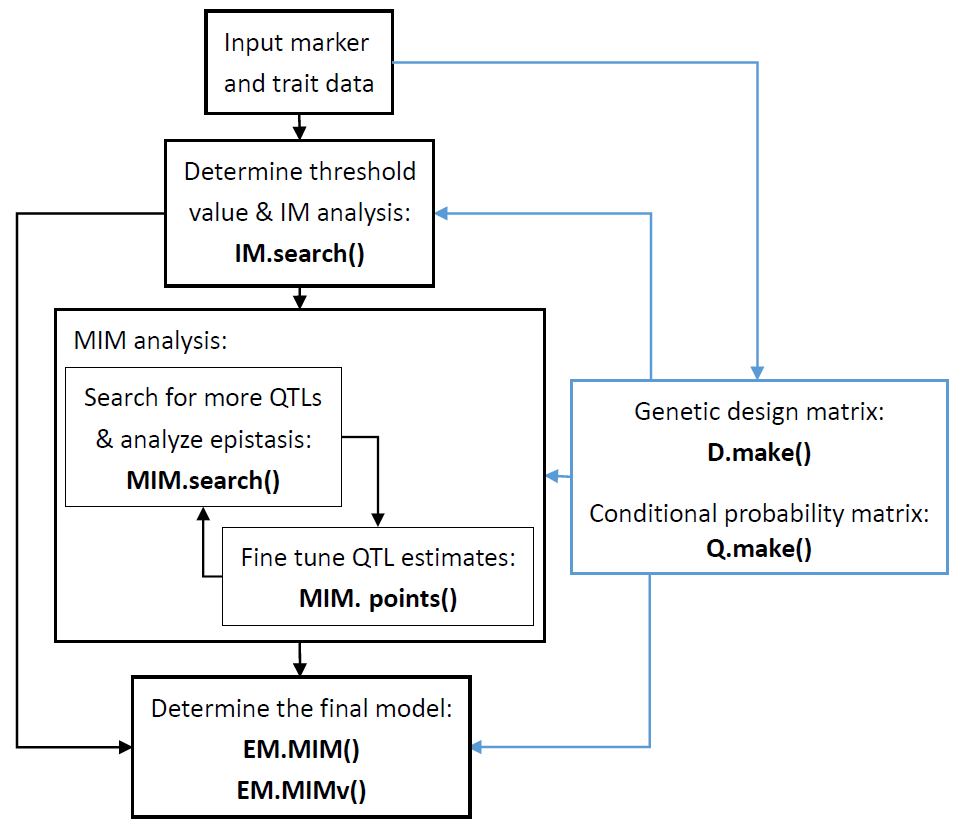
\includegraphics[width=0.9\linewidth]{figures/f0}
	\caption{Flowchart of using the QTL mapping functions in the QTLEMM package.}
	\label{f0}
\end{figure}

\begin{table}
	\centering
	\caption{The format example of marker/QTL information data}
	\label{t2}
	\centering
	\begin{tabular}[t]{ll}

		chromosome & position\_cM\\
		\toprule
		1 & 0\\
		1 & 24\\
		1 & 40\\
		... & ...\\
		12 & 72\\
		\addlinespace
		12 & 126\\
		\bottomrule
	\end{tabular}
\end{table}

\begin{table}
	\centering
	\caption{The format example of genotype data}
	\label{t3}
	\centering
	\resizebox{\ifdim\width>\linewidth\linewidth\else\width\fi}{!}{
		\begin{tabular}[t]{lccccccc}

			& $marker_1$ & $marker_2$ & $marker_3$ & $marker_4$ & $marker_5$ & ... & $marker_k$\\
			\toprule
			$ind_1$ & 2 & 1 & 1 & 2 & 0 & ... & 2\\
			$ind_2$ & 2 & 1 & 0 & 0 & 1 & ... & 1\\
			$ind_3$ & 2 & 2 & NA & 1 & 1 & ... & 0\\
			$ind_4$ & 0 & 0 & 1 & 0 & NA & ... & 2\\
			... & ... & ... & ... & ... & ... & ... & ...\\
			\addlinespace
			$ind_n$ & 1 & 1 & 0 & 0 & 1 & ... & 0\\
			\bottomrule
	\end{tabular}}
\end{table}

\subsection{Simulation examples}

Below a simulation example is presented to demonstrate the usage of the \CRANpkg{QTLEMM} package. Initially, it is necessary to install and load the \CRANpkg{QTLEMM} package and set an arbitrary random number seed, such as 8000, for data simulation in the R environment. Below are the codes. 

\begin{verbatim}
> install.packages("QTLEMM")
> library(QTLEMM)
> set.seed(8000)
> options(digits = 3)
\end{verbatim}

\subsubsection{Data generation}

\noindent The \code{progeny()} function can simulate marker genotype and phenotype (trait) data from experimental populations for QTL mapping analysis. This function accepts several key arguments: the \code{E.vector} argument represents the effects of the QTL; the \code{ng} argument specifies the generation number; the \code{h2} argument sets the heritability; the \code{size} argument contains the sample size; the \code{type} argument is used to specify the population type, which includes backcross (\code{type="BC"}), advanced intercross population (\code{type="AI"}), and recombinant inbred population (\code{type="RI"}). Now consider the scenario that a simulated dataset consists of 200 $F_2$ individuals with three chromosomes, each with eleven 10-cM equally spaced markers. Three QTLs are positioned at [1,23] (the 23 cM of the $1^{st}$ chromosome), [1,77] and [2,55], respectively, and their effects are assumed to be -10, 12, and 8, respectively. The $1^{st}$ and $3^{rd}$ QTLs have an additive-by-additive effect of 1. The heritability is set at 0.5. Below are the commands used to generate such a dataset. The command of defining the QTL effects is as follows:

\begin{verbatim}
> eff <- c("a1" = -10, "a2" = 12, "a3" = 8, "a1:a3" = 1)
\end{verbatim}

\noindent If other effects, such as dominance effect of 3 for the $2^{nd}$ QTL and additive-by-dominance effect of 2 for the $1^{st}$ and $2^{nd}$ QTLs, are considered, the arguments in the command is \code{d2=3} and \code{a2:d1=2}. Please refer to the \CRANpkg{QTLEMM} document in CRAN for more detailed instructions. The commands for setting the specified positions of QTLs and markers are as follows:

\begin{verbatim}
> marker <- cbind(rep(1:3,each = 11), rep(seq(0, 100, 10), 3))
> QTL <- cbind(c(1, 1, 2), c(23, 77, 55))
\end{verbatim}

\begin{figure}[th]
	\centering
	
\includegraphics[width=0.9\linewidth]{figures/f1}
	\caption{The graphical output generated by the \code{IM.search()} function. The upper plot shows the profile of LRT statistics, while the lower plot exhibits the profile of effects. The red line represents the threshold value of 9.62 obtained by using Gaussian process.}
	\label{f1}
\end{figure}

\noindent Then, the \code{progeny()} function can use the above commands to generate the QTL mapping data of 200 $F_2$ individuals with heritability 0.5.

\begin{verbatim}
> testdata <- progeny(QTL, marker, type = "RI", ng = 2, E.vector = eff, h2 = 0.5, 
  size = 200)
> names(testdata)
[1] "phe" "E.vector" "marker.prog" "QTL.prog" "genetic.value" "VG" "VE"
\end{verbatim}

\begin{verbatim}
> y <- testdata$phe
> geno <- testdata$marker.prog
\end{verbatim}

\noindent The \code{progeny()} function outputs a dataset into the object named \code{testdata}. This file contains four parts: phenotypes (\code{phe}), QTL effects (\code{E.vector}), marker genotypes (\code{marker.prog}), and QTL genotypes (\code{QTL.prog}). The markers and trait values of the 200 individuals in the \code{testdata} file are further extracted and organized into the \code{geno} matrix and \code{y} vector for QTL mapping analysis.

\subsubsection{Interval mapping} \label{3.2.2}

The \code{IM.search()} function is designed to implement the IM model for the QTL mapping analysis. Its arguments include: the \code{type} argument specifies the population type (\code{BC}, \code{AI}, and \code{RI} population); the \code{ng} argument represents the generation number; the speed argument determines the walking speed of the IM analysis (in cM); the \code{d.eff} argument indicates if the dominant effect will be considered or not (for AI or RI); the \code{QTLdist} argument specifies the minimum distance (in cM) between the detected QTL; the \code{plot.all} and \code{plot.chr} arguments indicate whether plots of the LRT statistic profile will be generated or not. Below are the codes of using the \code{IM.search()} function to perform the IM analysis on the simulated dataset without considering any dominance effect.

\begin{verbatim}
> IMtest <- IM.search(marker, geno, y, type = "RI", ng = 2, speed = 1, d.eff = FALSE, 
  QTLdist = 15, plot.all = TRUE, plot.chr = FALSE, console = FALSE)
> names(IMtest)
[1] "effect" "LRT.threshold" "detect.QTL" "model" "inputdata"  
\end{verbatim}

\begin{verbatim}
> IMtest$LRT.threshold
 95%
9.62
\end{verbatim}

\noindent The outputs of the \code{IM.search()} function (\code{IMtest}) include: estimated effects at all positions (\code{effect});  LRT threshold (\code{LRT.threshold}) obtained using Gaussian process; numerical results of the detected QTLs (\code{detect.QTL}); graphical outputs. The \code{IM.search()} function can also perform the REG IM model for the QTL mapping analysis by setting the argument \code{method=”REG”} (default \code{method=”EM”}). Figure~\ref{f1} is the graphical output of the \code{IM.search()} function. It illustrates the profiles of the LRT statistics and effects across the three chromosomes. The LRT profile shows three significant peaks, indicating three QTLs are detected, on two of the three chromosomes. For this dataset, the LRT threshold of considering both additive and dominance effects for assessing the significance of QTL detection is 12.58 (12.15) by using Gaussian process (permutation test in R/\CRANpkg{qtl}). The LRT threshold value of considering only additive effect is 9.62 (9.82) by using Gaussian process (using our own permutation program, as R/\CRANpkg{qtl} does not provide the option of considering only additive effect in the F2 population). The numerical results of the detected QTLs can be listed using the following commands.

\begin{verbatim}
> detQTL <- IMtest$detect.QTL
> detQTL
   chr cM    a1  LRT     R2
14   1 14 -7.00 24.1 0.1064
77   1 77  8.03 29.6 0.1324
153  2 53  6.14 17.3 0.0787
\end{verbatim}

\noindent The IM analysis concludes that the three QTLs are detected at [1,14], [1,77] and [2,53] with effects of -7.00, 8.03 and 6.14, respectively. They contribute approximately 10.64\%, 13.24\%, and 7.87\% of the trait variation, respectively. 

\subsubsection{Multiple interval mapping}

The analysis of the IM model can be further improved using the MIM approach by jointly fitting the three QTL into the model so as to obtain more precise and accurate estimates of QTL parameters. The \code{EM.MIM()} function is designed to perform the MIM model analysis. Before conducting the \code{EM.MIM()} function, two matrices, the genetic design matrix (\code{D.matrix}) and the conditional probability matrix (\code{cp.matrix}), must be constructed first. The \code{D.make()} and \code{Q.make()} functions are utilized to generate the two matrices, respectively. The commands in the \code{D.make()}, \code{Q.make()} and \code{EM.MIM()} functions for the MIM model fitting the three QTL at [1,14], [1,77] and [2,53] with an additive by additive effect (between the QTLs at [1,14] and [2,53]) are given below respectively.

\begin{verbatim}
> dQTL <- detQTL[,1:2]
> D.matrix <- D.make(nQTL = 3, type = "RI", a = TRUE, d = 0, aa = c(1, 3))
\end{verbatim}

\noindent The first argument of the \code{D.make()} function is the number of QTL in the MIM model and is \code{nQTL=3} in this case; the second argument specifies the population type and is \code{type="RI"}; the arguments \code{a} and \code{d} indicate if additive or dominance effects will be considered and they are \code{a=TRUE} and \code{d=0} since only the additive effects are considered; the arguments \code{aa}, \code{dd}, and \code{ad} specify the epistatic effects between QTLs and is \code{aa=c(1, 3)} since the additive by additive effect between the $1^{st}$ and $3^{rd}$ QTLs is considered. The dimension of \code{D.matrix} matrix for this three-QTL MIM model is $27\times 4$, and the elements of first six rows are shown below.

\begin{verbatim}
> dim(D.matrix)
[1] 27 4
\end{verbatim}

\begin{verbatim}
> head(D.matrix)
    a1 a2 a3 a1:a3
222  1  1  1     1
221  1  1  0     0
220  1  1 -1    -1
212  1  0  1     1
211  1  0  0     0
210  1  0 -1    -1
\end{verbatim}

\noindent The arguments in the \code{Q.make()} function for generating the conditional probability matrix of the three-QTL MIM model in this case are shown below. The dimension of the \code{cp.matrix} matrix for this three-QTL MIM model is $200\times 27$.

\begin{verbatim}
> cp.matrix <- Q.make(dQTL, marker, geno, type = "RI", ng = 2)$cp.matrix
> dim(cp.matrix)
[1] 200 27
\end{verbatim}

Three inputs are required for driving the \code{EM.MIM()} function to perform the MIM analysis: the genetic design matrix (\code{D.matrix}); the conditional probability matrix (\code{cp.matrix}); the phenotypic values (\code{y}). The outputs from the \code{EM.MIM()} function include a vector containing the estimated QTL effects (\code{E.vector}), the mean (\code{beta}), the residual variance (\code{variance}), the posterior probabilities matrix (\code{PI.matrix}), the log likelihood value (\code{log.likelihood}), the LRT statistics (\code{LRT}), the coefficient of determination (\code{R2}), the estimated trait values (\code{y.hat}), and the iteration time (\code{iteration.time}) as shown below.

\begin{verbatim}
> MIMtest <- EM.MIM(D.matrix = D.matrix, cp.matrix = cp.matrix, y = y, console = FALSE)
> names(MIMtest)
[1] "QTL" "E.vector" "beta" "variance" "PI.matrix" "log.likelihood" "LRT" "R2"              
[9] "y.hat" "yu.hat" "iteration.number" "model"
\end{verbatim}

\begin{verbatim}
> MIMtest$E.vector
   a1    a2   a3 a1:a3
-9.61 10.29 6.35  1.66
\end{verbatim}

\begin{verbatim}
> c(MIMtest$log.likelihood, MIMtest$LRT, MIMtest$R2)
[1] -772.192  145.114  0.411
\end{verbatim}

\noindent The log likelihood of the MIM model fitting the three QTL with epistasis is approximately -772. The estimated QTL effects are approximately -9.61, 10.29 and 6.35 (true values being -10, 12, and 8), respectively, and the estimated epistatic effect is approximately 1.66. The estimated heritability (\code{R2}) is 0.411, while the true heritability is 0.50. The above MIM-related functions can also perform the REG IM model (multiple QTL version) by setting the argument \code{method=”REG”}. Besides using the original marker and trait data, note especially that all the MIM-related functions can utilize the results from the analysis of IM or MIM functions, such as the \code{IM.search()}, \code{MIM.search()}, and \code{MIM.points()} functions, as input to conduct the analysis. Also, the marker and trait data and the detected QTL information in the previous analysis can be used in the subsequent analysis. Below are the codes of using the results from the IM analysis (\code{IMtest}) to conduct the \code{EM.MIM()} function..

\begin{verbatim}
> MIMtest_ <- EM.MIM(D.matrix = D.matrix, IMresult = IMtest, console = FALSE)
> MIMtest_$E.vector
   a1    a2   a3 a1:a3
-9.61 10.29 6.35  1.66
\end{verbatim}

The \code{EM.MIMv()} function can provide the asymptotic variance-covariance matrix of the QTL estimates. The inputs in the \code{EM.MIMv()} function include: QTL information about the QTL effects and positions (\code{QTL}); marker information (\code{marker}); genotypes (\code{geno}); genetic design matrix (\code{D.matrix}); conditional probability matrix (\code{cp.matrix}); phenotypic values (\code{y}). If the argument \code{cp.matrix} is set to \code{NULL}, the conditional probability matrix is constructed from the input QTL information and marker information. If the estimated QTL positions coincide with markers, the asymptotic variance-covariance matrix is not available. Below are the arguments of the \code{EM.MIMv()} function using the marker and trait data to produce the variance-covariance matrix for the MIM model fitting the three detected QTLs at [1,14], [1,77], and [2,53].

\begin{verbatim}
> MIMv <- EM.MIMv(dQTL, marker, geno, D.matrix, cp.matrix = NULL, y, console = FALSE) 
> # MIMv <- EM.MIMv(D.matrix = D.matrix, IMresult = IMtest, console = FALSE)
> names(MIMv)
[1] "E.vector" "beta" "variance" "PI.matrix" "log.likelihood" "LRT" "R2" "y.hat"
[9] "iteration.number" "avc.matrix" "EMvar"
\end{verbatim}

\noindent The \code{avc.matrix} is the asymptotic variance-covariance matrix, and the \code{EMvar} contains the asymptotic variances of the estimates. They are listed below.

\begin{verbatim}
> round(MIMv$avc.matrix, 3)
           QTL1   QTL2   QTL3     a1     a2     a3  a1:a3 residual.var     mu
QTL1      0.015  0.017  0.013 -0.003  0.000  0.014  0.076       -0.073 -0.003
QTL2      0.017  0.004 -0.006 -0.023  0.021 -0.003  0.041       -0.191  0.002
QTL3      0.013 -0.006  0.065 -0.034  0.035  0.036  0.134       -0.688  0.009
a1       -0.003 -0.023 -0.034  1.417 -0.354 -0.091  0.038        1.775  0.006
a2        0.000  0.021  0.035 -0.354  1.585 -0.039  0.154       -2.462 -0.096
a3        0.014 -0.003  0.036 -0.091 -0.039  1.463  0.257       -1.185 -0.034
a1:a3     0.076  0.041  0.134  0.038  0.154  0.257  3.724       -2.787 -0.096
variance -0.073 -0.191 -0.688  1.775 -2.462 -1.185 -2.787      179.411  0.030
X1       -0.003  0.002  0.009  0.006 -0.096 -0.034 -0.096        0.030  0.650
\end{verbatim}

\begin{verbatim}
> round(MIMv$EMvar, 3)
 QTL1  QTL2  QTL3    a1    a2    a3  a1:a3 residual.var     mu
0.015 0.004 0.065 1.417 1.585 1.463  3.724      179.411  0.650
\end{verbatim}

\noindent The asymptotic variances of the estimated QTL positions and effects are 0.015, 0.004, 0.065, 1.417, 1.585, 1.463 and 3.724, respectively. The asymptotic variances of the estimated mean and residual variance are 0.650 and 179.411, respectively.

The \code{MIM.search()} function is devised to fit the detected QTLs into the model to search the genome for other possible QTL. The arguments in the \code{MIM.search()} function include the detected QTL (denoted by \code{dQTL2} in this example), \code{marker} (for marker information), \code{geno} (for genotypes), \code{y} (for phenotypes), \code{type} (for population type), \code{ng} (for the generation number), \code{D.matrix} (for the genetic design matrix), \code{speed} (for the walking speed in cM), \code{QTLdist} (for the minimum distance between detected QTLs). The outputs of the \code{MIM.search()} function include information about the estimates of all search positions (\code{effect}), the best QTL positions with the largest log likelihood (\code{QTL.best}), and the estimated QTL effects at the best QTL positions (\code{effect.best}). For demonstration purposes, assume that the two detected QTLs located at [1,14] and [1,77] are fitted into the MIM model to search for the next (third) QTL considering the additive by additive effect (the design matrix will be the same as that in the above \code{EM.MIM()} function). Below are the commands of the \code{MIM.search()} function to conduct the search for the third QTL given the two detected QTLs:

\begin{verbatim}
> dQTL2 <- cbind(c(1, 1), c(14, 77))
> MIMs <- MIM.search(dQTL2, marker, geno, y, type = "RI", ng = 2, D.matrix = D.matrix,
  speed = 1, QTLdist = 15, console = FALSE)
> names(MIMs)
[1] "effect" "QTL.best" "effect.best" "model" "inputdata"  
\end{verbatim}

\begin{verbatim}
> MIMs$QTL.best
        chromosome position(cM)
QTL 1            1           14
QTL 2            1           77
QTL new          2           54
\end{verbatim}

\begin{verbatim}
> MIMs$effect.best
    a1     a2    a3  a1:a3     LRT log.likelihood    R2
-9.619 10.302 6.385  1.806 145.876       -772.129 0.412
\end{verbatim}

\noindent The third QTL is detected at the position [2,54] with an estimated effect of approximately 6.385. The log likelihood of the MIM model is about -772.129. The LRT statistic for testing the significance of the effects jointly is about 145.876. 

Another function related to the MIM analysis is the \code{MIM.points()} function, which is used to fine tune the estimation of QTL parameters by multidimensional search around the detected QTLs. The fine-tuning ranges around the detected QTLs are defined using the scope argument, while the other arguments are the same as those in the \code{MIM.search()} function. Below is the command of the \code{MIM.search()} function for performing a three-dimensional search on the 10-cM range on both sides of the three QTL at [1,14], [1,77] and [2,54] (with additive by additive effect).

\begin{verbatim}
> MIMp <- MIM.points(dQTL, marker, geno, y, type = "RI", ng = 2, D.matrix = D.matrix, 
  speed = 2, scope = 10, console = FALSE)
> # MIMp <- MIM.points(D.matrix = D.matrix, speed = 2, scope = 10, IMresult = IMtest,
  console = FALSE)
> names(MIMp)
[1] "effect" "QTL.best" "effect.best" "model" "inputdata"  
\end{verbatim}

\begin{verbatim}
> MIMp$QTL.best
     chromosome position(cM)
[1,]          1           24
[2,]          1           75
[3,]          2           53
\end{verbatim}

\begin{verbatim}
> MIMp$effect.best
     a1     a2    a3  a1:a3     LRT log.likelihood    R2
-10.846 11.994 6.503  3.725 181.130       -765.371 0.464
\end{verbatim}

\noindent The results show that the largest model log likelihood becomes -765.371, and the estimated heritability is 0.464. After fine-tuning, the detected positions are closer to the true positions [1,23], [1,77] and [2,55], compared to the estimated positions [1,14], [1,77] and [2,53] before fine-tuning. With these estimates, other composite genetic parameters such as heritability and variance components of a quantitative trait can be estimated. Additionally, the response to selection can be predicted based on these estimates.

\subsection{The yeast dataset example}

The yeast dataset \citep{Brem-2005} consists of 112 backcross individuals with 5740 traits and 1072 markers. The raw data are reprocessed into a new dataset called `yeast.process`, which can be loaded from \CRANpkg{QTLEMM} package using the following command:

\begin{verbatim}
> load(system.file("extdata", "yeast.process.RDATA", package = "QTLEMM"))
\end{verbatim}

\noindent The \code{yeast.process} dataset comprises three lists: the list of marker genotypes (\code{yeast.process\$geno}) that contains the marker genotypes of the 112 individuals; the list of trait values (\code{yeast.process\$pheno}) that contains the trait values of the 112 individuals; the list of marker information (\code{yeast.process\$marker}) that includes the marker map (distances) of the 1072 markers on the 16 chromosomes.

\begin{verbatim}
> geno <- yeast.process$geno
> marker <- yeast.process$marker
> pheno <- yeast.process$pheno
\end{verbatim}

\subsubsection{Selective genotyping data}

For the demonstration of analyzing selective genotyping data, we selected the $3590^{th}$ trait from the dataset and intentionally deleted the marker genotypes of the individuals with medium trait values to produce selective genotyping data for QTL mapping analysis. Specifically, one half of the individuals with extreme trait values (comprising one quarter each from the upper and lower extremes) are chosen to keep their marker genotypes and trait values, and the marker genotypes of the remaining individuals are deleted and ignored in the analysis. Below are the codes for generating the selective genotyping dataset.

\begin{verbatim}
> y0 <- pheno[, 3590]
> y <- y0[y0>quantile(y0)[4] | y0<quantile(y0)[2]]
> yu <- y0[y0 >= quantile(y0)[2] & y0 <= quantile(y0)[4]]
> geno.s <- geno[y0 > quantile(y0)[4] | y0 < quantile(y0)[2],]
\end{verbatim}

\begin{figure}[htbp]
	\centering
	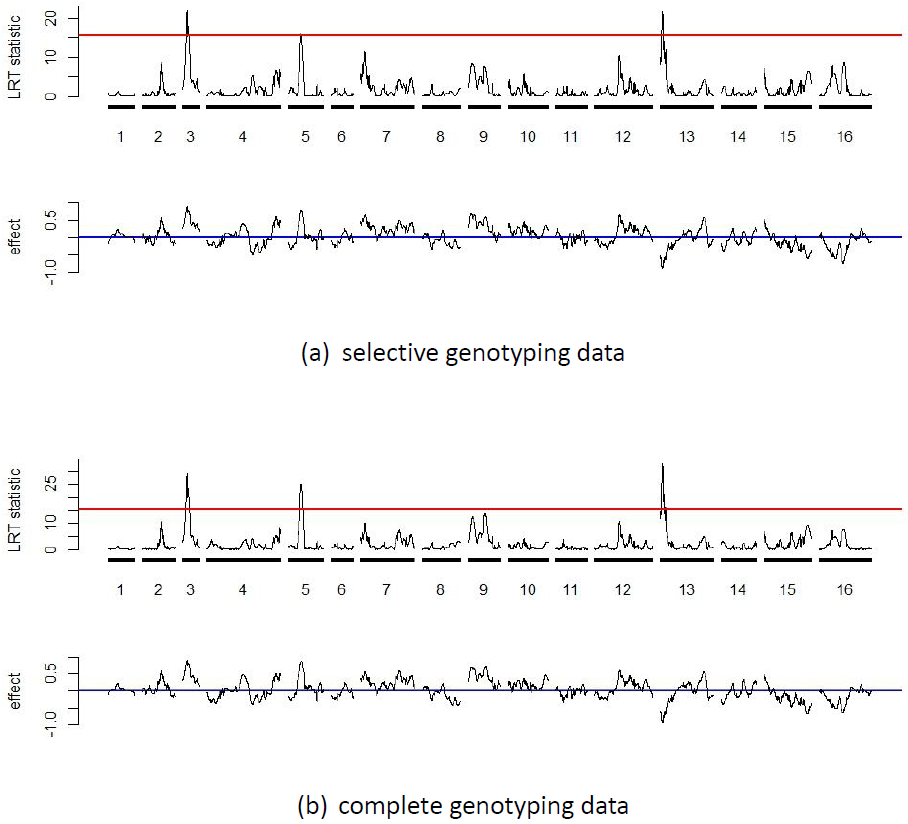
\includegraphics[width=0.8\linewidth]{figures/f2}
	\caption{The profiles of the LRT statistics and estimated effects along the genome by using the \code{IM.search2()} function to analyze the selective genotyping data of the $3590^{th}$ trait (part a), and using the \code{IM.search()} function to analyze the complete genotyping data (part b). The red line indicates the LRT threshold obtained by using Gaussian process for assessing the significance of QTL detection.}
	\label{f2}
\end{figure}

\noindent The vector \code{y} contains the trait values of the individuals with marker genotypes (the upper and lower 25\% individuals), and the \code{geno.s} argument consists of their marker genotypes. The vector \code{yu} contains the trait values of individuals without marker genotypes. The \code{IM.search()} function can also perform several selective genotyping QTL mapping methods, which encompass the \citeauthor{Lee-2014} model (\code{sele.g="f"}), the truncated model (\code{sele.g="t"}), and the population frequency-based model (\code{sele.g="p"}), to analyze the selective genotyping dataset (see \citeauthor{Lee-2014} \citeyear{Lee-2014} for details). If \code{sele.g="n"}, the function is used to analyze the complete genotyping data.

\subsubsection{Selective genotyping IM and MIM analysis} \label{3.3.2}

The followings are the codes of the \code{IM.search()} function to analyze the selective genotyping data of the $3590^{th}$ trait. The random number seed 8000 is used to set up the Gaussian process to compute threshold values for assessing the significance of QTLs.

\begin{verbatim}
> library(QTLEMM) 
> set.seed(8000)
> IMtest2 <- IM.search(marker, geno.s, y, yu, sele.g = "f", type = "BC", ng = 1, 
  plot.all = TRUE, plot.chr = FALSE, console = FALSE)
> IMtest2$detect.QTL
     chr  cM     a1  LRT     R2
626    3  53  0.893 22.0 0.1128
1579   5 112  0.753 16.0 0.0749
4523  13  22 -0.882 21.7 0.1048
> IMtest2$LRT.threshold
 95% 
15.4 
\end{verbatim}

\noindent Figure~\ref{f2}(a) presents the profiles of the LRT statistics and estimated effects along the genome. It shows that three QTL are detected at [3,53], [5,112] and [13,22], respectively. The LRT threshold value is 15.40 (15.36) by the Gaussian process (permutation test in R/\CRANpkg{qtl}). For comparison, we  use the \code{IM.search()} function to conduct complete genotyping analysis for the $3590^{th}$ trait.

\begin{verbatim}
> IMcon <- IM.search(marker, geno, y0, type = "BC", ng = 1, LRT.thre = 15.4,
  plot.all = TRUE, plot.chr = FALSE, console = FALSE)
> IMcon$detect.QTL
     chr  cM     a1  LRT    R2
624    3  53  0.904 29.0 0.210
1580   5 117  0.877 25.0 0.171
4511  13  22 -0.945 33.1 0.231
\end{verbatim}

\noindent The profiles of the LRT statistics and estimated effects along the genomes are presented in Figure~\ref{f2}(b). It shows that three QTL are detected at [3,53], [5,115] and [13,22], respectively. Both the selective and complete genotyping IM analyses produce similar LRT statistic profiles and estimates of positions and effects. For each detected QTL, the complete genotyping data analysis produces larger LRT statistics and $R^{2}$’s as compared to the selective genotyping analysis.

Using the \code{IM.search()} function, the estimates of QTL effects and positions, model likelihoods and model $R^{2}$ values were obtained individually. Certainly, we would like to further fit these detected QTLs simultaneously into a multiple-QTL model (the MIM Model). This allows the QTLs to be jointly fitted and controlled in the model to explain more genetic variation of the quantitative traits and obtain more precise estimates. Below are the commands of the \code{EM.MIM()} function to perform the selective genotyping MIM model analysis that considers the three detected QTLs and their all possible epistasis.

\begin{verbatim}
> D.matrix <- D.make(3, type = "BC", aa = TRUE)
> MIMtest2 <- EM.MIM(D.matrix = D.matrix, IMresult = IMtest2, console = FALSE)
> MIMtest2$E.vector
   a1    a2     a3  a1:a2  a1:a3  a2:a3
0.818 0.744 -0.954 -0.641  0.371 -0.423
\end{verbatim}

\begin{verbatim}
> c(MIMtest2$log.likelihood, MIMtest2$LRT, MIMtest2$R2)
[1] -115.253  79.117  0.512
\end{verbatim}

\noindent The model $R^{2}$ and likelihood are 0.512 and -115.41, respectively. The estimated marginal and epistatic QTL effects are 0.818, 0.744, -0.954, -0.641, 0.371 and -0.423, respectively. The \code{MIM.points()} function can be further used to perform a multi-dimensional search around the 5-cM regions of the detected QTL positions (at [3,53], [5,112] and [13,22]) to fine-tune the QTL estimates (using the argument of \code{scope=5}). Below are the codes of the \code{MIM.points()} function to perform the multi-dimensional search and the fine-tuning results.

\begin{verbatim}
> MIMp <- MIM.points(D.matrix = D.matrix, scope = 5, IMresult = IMtest2, console = FALSE)
> MIMp$QTL.best
     chromosome position(cM)
[1,]          3           58
[2,]          5          111
[3,]         13           21
\end{verbatim}

\begin{verbatim}
> MIMp$effect.best
   a1    a2     a3  a1:a2  a1:a3  a2:a3    LRT log.likelihood    R2
0.678 0.758 -0.964 -0.866  0.673 -0.499 82.214       -113.705 0.524
\end{verbatim}

\noindent The model with the largest log likelihood (-113.705) occurs at positions [3,58], [5,111] and [13,21], and the estimated effects are 0.678, 0.758, -0.964, -0.866, 0.673, -0.499, respectively. The model $R^{2}$ (estimated heritability) improves from 0.512 to 0.524. 

\section{Using QTLEMM for QTL hotspot detection}

The analysis of QTL hotspot detection has been a pivotal step towards unraveling the genetic architectures of quantitative traits in the study of genes, genomes and genetics \citep{Breitling-2008, Fu-2009, Neto-2012, Wang-2014, Yang-2019, Wu-2021}. The genetical genomics experiments and public QTL databases are two feasible sources to provide data with many QTLs for the detection of QTL hotspots. The statistical framework of QTL hotspot detection proposed by \citet{Yang-2019} and \citet{Wu-2021} is capable of accommodating both types of data. The framework addresses various challenges, including handling the correlation structure among traits, identifying different types of hotspots, and ensuring computational efficiency, thereby making it practical for QTL hotspot detection. The \CRANpkg{QTLEMM} package offers the statistical framework by \citeauthor{Yang-2019} and \citeauthor{Wu-2021} for the detection of QTL hotspots. The functions for detecting QTL hotspots using the framework are summarized in Table~\ref{t4}. Below, we present the analyses of two real examples, the yeast genetic genomics dataset and the GRAMENE rice database, as demonstration of using these functions for detecting QTL hotspots.

\subsection{The yeast genetic genomics dataset example}

There are 5740 molecular traits in the yeast dataset \citep{Brem-2005}. The QTL mapping procedure employed for the $3590^{th}$ trait using the \code{IM.search()} function can be applied to analyze the remaining 5739 traits, obtaining their LRT statistics at all positions along the genome. These LRT statistics can then be converted into LOD scores using the formula $LOD = LRT / 4.6$. Subsequently, the LOD scores are organized into a LOD matrix for QTL hotspot detection, following the methods outlined by \citet{Yang-2019} and \citet{Wu-2021}. The \code{LOD.QTLdetect()} function is constructed to detect QTL hotspots. It requires two input datasets: the LOD matrix and the bin information on the chromosomes. The LOD matrix is a $t\times p$ matrix, where $t$ and $p$ are the numbers of traits and numbers of bins on the chromosomes, respectively. The LOD matrix contains the LOD scores of all bins for all traits (refer to Table~\ref{t5}). The bin information is an $n\times2$ matrix, where $n$ is the number of chromosomes, and it contains the information about the bin number on each chromosome. The first column denotes the chromosomes, and the second column denotes the numbers of bins on the chromosomes (refer to Table~\ref{t6}).

\begin{table}[hbt]
	\centering
	\caption{List of the functions for QTL hotspot detection in the QTLEMM package}
	\label{t4}
	\centering
	\begin{tabular}[t]{>{}l>{\raggedright\arraybackslash}p{30em}}
		\toprule
		Function & Description\\
		\midrule
		\code{LOD.QTLdetect()} & Detect QTL by LOD matrix.\\
		\code{EQF.permu()} & EQF matrix cluster permutation process for QTL hotspot detection.\\
		\code{EQF.plot()} & Depict the EQF plot by the result of permutation process.\\
		\code{Qhot()} & This function generates both numerical and graphical summaries of the QTL hotspot detection in the genomes.\\
		\code{Qhot.EQF()} & Convert the QTL flanking marker data to EQF matrix and carry out the EQF matrix cluster permutation process.\\
		\bottomrule
	\end{tabular}
\end{table}

\begin{table}
	\centering
	\caption{The format of LOD matrix}
	\label{t5}
	\centering
	\resizebox{\ifdim\width>\linewidth\linewidth\else\width\fi}{!}{
		\begin{tabular}[t]{lccccccc}

			& $bin_1$ & $bin_2$ & $bin_3$ & $bin_4$ & $bin_5$ & ... & $bin_n$\\
			\toprule
			$trait_1$ & 0.047 & 0.116 & 0.209 & 0.313 & 0.342 & ... & 0.358\\
			$trait_2$ & 0.095 & 0.176 & 0.274 & 0.376 & 0.301 & ... & 0.342\\
			$trait_3$ & 0.798 & 0.67 & 0.533 & 0.394 & 0.342 & ... & 0.284\\
			$trait_4$ & 0.363 & 0.321 & 0.272 & 0.219 & 0.192 & ... & 0.149\\
			$trait_5$ & 0.017 & 0.01 & 0.005 & 0.002 & 0.001 & ... & 0\\
			\addlinespace
			... & ... & ... & ... & ... & ... & ... & ...\\
			$trait_t$ & 0.683 & 0.593 & 0.471 & 0.336 & 0.304 & ... & 0.271\\
			\bottomrule
	\end{tabular}}
\end{table}

\begin{table}
	\centering
	\caption{The format example of bin information}
	\label{t6}
	\centering
	\begin{tabular}[t]{ll}

		chromosome & number\_of\_bin\\
		\toprule
		1 & 256\\
		2 & 324\\
		3 & 160\\
		4 & 723\\
		... & ...\\
		\addlinespace
		15 & 463\\
		16 & 513\\
		\bottomrule
	\end{tabular}
\end{table}

The LOD matrix of the yeast data can be downloaded from GitHub using the commands below. Users can combine the four files (\code{yeast.LOD.1.RDATA}, \code{yeast.LOD.2.RDATA}, \code{yeast.LOD.3.RDATA}, \code{yeast.LOD.4.RDATA}) to obtain the complete LOD matrix.

\begin{verbatim}
> load(url("https://github.com/py-chung/QTLEMM/raw/main/inst/extdata/yeast.LOD.1.RDATA"))
> load(url("https://github.com/py-chung/QTLEMM/raw/main/inst/extdata/yeast.LOD.2.RDATA"))
> load(url("https://github.com/py-chung/QTLEMM/raw/main/inst/extdata/yeast.LOD.3.RDATA"))
> load(url("https://github.com/py-chung/QTLEMM/raw/main/inst/extdata/yeast.LOD.4.RDATA"))
> load(url("https://github.com/py-chung/QTLEMM/raw/main/inst/extdata/yeast.LOD.bin.RDATA"))
> LOD <- rbind(yeast.LOD.1, yeast.LOD.2, yeast.LOD.3, yeast.LOD.4)
> bin <- yeast.LOD.bin
\end{verbatim}

\noindent Once the LOD matrix is available, the \code{LOD.QTLdetect()} function can be applied to detect QTL hotspots. The function's arguments include \code{LOD} for the LOD matrix (refer to Table~\ref{t5}), \code{bin} for the numbers of bins on each chromosome (refer to Table~\ref{t6}), \code{thre} for the threshold value (in terms of LOD) of QTL detection, and \code{QTLdist} for specifying the minimum distance (cM) between the detected QTL. The numerical results of this function will be output to the \code{LOD.QTLdetect.result} file.

\begin{verbatim}
> library(QTLEMM)
> set.seed(8000)
> LOD.QTLdetect.result <- LOD.QTLdetect(LOD, bin, thre = 3, QTLdist = 20, console = FALSE)
> names(LOD.QTLdetect.result)
[1] "detect.QTL.number" "QTL.matrix" "EQF.matrix" "linkage.QTL.number"
[5] "LOD.threshold" "bin"
\end{verbatim}

\noindent The \code{LOD.QTLdetect.result} file is a data list comprising several components: \code{detect.QTL.number} contains the number of detected QTL of each trait; \code{QTL.matrix} holds the QTL positions, where elements marked as 1 represent the QTL positions, elements marked as 0 represent bins with LOD scores under the LOD threshold, and other positions are designated as NA; \code{EQF.matrix} contains the EQF value of each bin; \code{linkage.QTL.number} indicates the number of linked QTL among all detected QTLs; \code{LOD.threshold} and \code{bin} remain the same as those in the input data. With these information, the \code{EQF.permu()} function embedding the permutation analysis \citep[with trait grouping;][]{Wu-2021} can be applied to detect QTL hotspots. The arguments in the \code{EQF.permu()} function involve inputting the output data from \code{LOD.QTLdetect()}, specifying the permutation time (\code{npermu}), and using the genome-wide error rate (GWER) of a given level $\alpha$ to carry out the permutation analysis. Additionally, the \code{Q=TRUE} argument is to perform permutation analysis without trait grouping.

\begin{verbatim}
> EQF.permu.result <- EQF.permu(LOD.QTLdetect.result, npermu = 1000, alpha = 0.05, 
  Q = TRUE, console = FALSE)
> names(EQF.permu.result)
[1] "EQF.matrix" "bin" "LOD.threshold" "cluster.number" "cluster.id" "cluster.matrix"
[7] "permu.matrix.cluster" "permu.matrix.Q" "EQF.threshold"
\end{verbatim}

The output of the \code{EQF.permu()} function includes several components. The \code{EQF.matrix}, \code{bin}, and \code{LOD.threshold} lists represent the EQF matrix, bin information matrix, and the LOD threshold respectively, which are the same as those in the input data. The \code{cluster.number} contains the number of QTLs in each trait group. The \code{cluster.id} contains the serial number of traits in each trait group. The \code{cluster.matrix} includes the reduced EQF matrix after trait grouping. The \code{permu.matrix.cluster} contains the result of permutation with trait grouping, sorted by order. Similarly, the \code{permu.matrix.Q} contains the result of the permutation without trait grouping, also sorted by order. The \code{EQF.threshold} represents the EQF threshold calculated from the permutation analysis. Moreover, the \code{EQF.plot()} function is designed to plot the figure of the EQF architecture of the genome (see Figure~\ref{f3}) using the output of the \code{EQF.permu()} function. Below are the codes.

\begin{verbatim}
> EQF.plot(EQF.permu.result, plot.all = TRUE, plot.chr = FALSE)
\end{verbatim}

\noindent The command of \code{plot.all = TRUE} is to draw the EQF architecture of the entire genome (16 chromosomes) in a single figure (Figure~\ref{f3}). If \code{plot.chr = TRUE}, the EQF architectures of genome is drawn separately by chromosomes in different figures. 

\subsection{The GRAMENE rice database example}

The \code{Qhot()} function manages summarized QTL data collected from public QTL databases to detect QTL hotspots. Below, we demonstrate the use of the \code{Qhot()} function to detect QTL hotspots using the public GRAMENE rice database. First the QTL data in the GRAMENE rice database can be loaded from \CRANpkg{QTLEMM} package using the following command:

\begin{verbatim}
> load(system.file("extdata", "gramene.chr.RDATA", package = "QTLEMM"))
> load(system.file("extdata", "gramene.QTL.RDATA", package = "QTLEMM"))
> head(gramene.chr)
  CHR Center.cM. Length.cM.
1   1      74.2         184
2   2      55.5         161
3   3      84.3         166
4   4      19.7         133
5   5      51.8         121
6   6      66.8         127
\end{verbatim}

\begin{figure}[htbp]
	\centering
	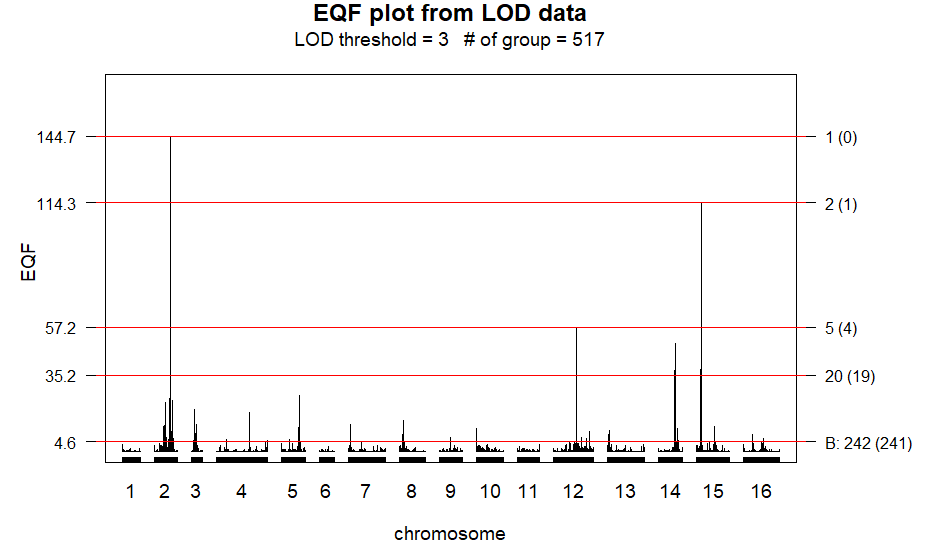
\includegraphics[width=0.95\linewidth]{figures/f3}
	\caption{The 3-LOD EQF architecture of the yeast 16 chromosomes and the hotspots detected under different EQF thresholds at GWER of 5\% by using the \code{EQF.plot()} function with the output of the \code{EQF.permu()} function. The EQF architecture are constructed by the uniform method with bin size of 0.5 cM.}
	\label{f3}
\end{figure}

\begin{figure}[htbp]
	\centering
	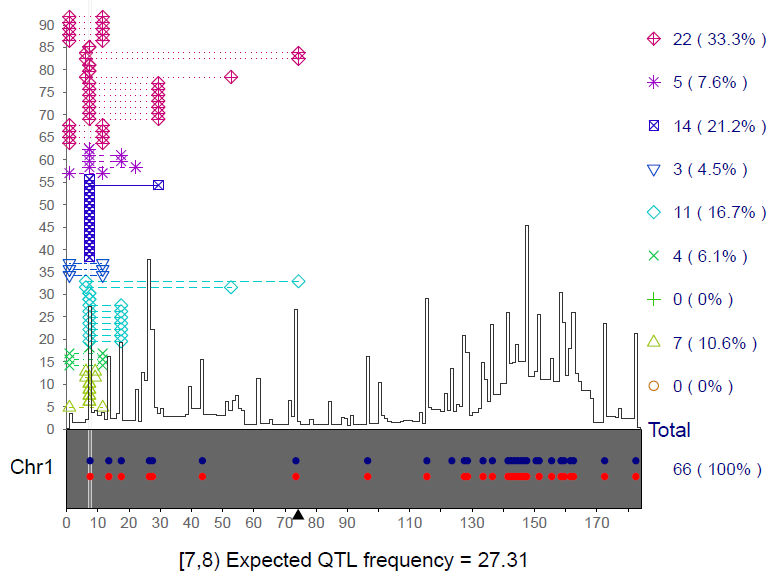
\includegraphics[width=1\linewidth]{figures/f4}
	\caption{The plot of EQF architecture of the 1st chromosome and breakdown of QTL composition at bin [7,8) in the PDF file produced by using the \code{Qhot()} function with \code{save.pdf=TRUE}. The x-axis denotes the $1^{st}$ chromosome, the y-axis denotes the EQF values. The black triangle denotes the position of centromere. The blue (red) dots denote the QTL hotspots detected by the \citet{Yang-2019} method (the Q method). The 9 different colored symbols denote the QTLs responsible for the 9 different trait categories \citep[see][]{Yang-2019}. The dotted lines denote the lengths of the marker intervals flanking the QTLs (QTL intervals). In total, 66 QTLs contribute probabilities to the EQF value of 27.31 at bin [7,8). The numbers of contributive QTLs of the 9 different trait categories are 22, 5, 14, 3, 11, 4, 0, 7, and 0, respectively.}
	\label{f4}
\end{figure}

\begin{figure}[htbp]
	\centering
	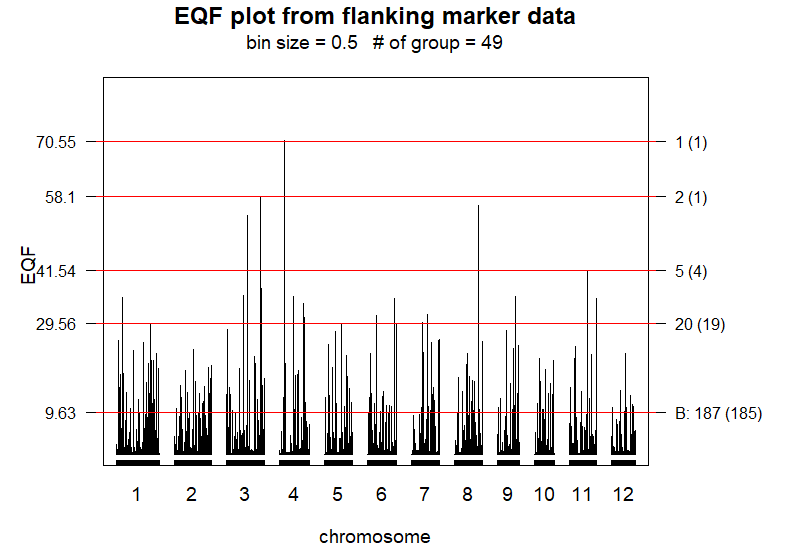
\includegraphics[width=0.9\linewidth]{figures/f5}
	\caption{The EQF architectures of the rice 12 chromosomes and the hotspots detected under different EQF thresholds at GWER of 5\% by using the EQF.plot() function with the output of the \code{Qhot.EQF()} function. The EQF architecture are constructed by the uniform method with bin size of 0.5 cM.}
	\label{f5}
\end{figure}

\begin{verbatim}
> head(gramene.QTL) # 9 trait categories in the second column
  X       Trait chr     L     R
1 1 Biochemical   1  54.1  54.1
2 2       Vigor   1 147.4 147.4
3 3       Vigor   1 147.4 147.4
4 4       Vigor   1 147.4 147.4
5 5       Vigor   1 147.4 158.6
6 6       Vigor   1  54.1  54.1
\end{verbatim}

\noindent The \code{gramene.chr} is a data frame containing the information about the chromosomes, including their numbers, midpoint positions (in cM), and lengths. The \code{gramene.QTL} is a data frame for the information about QTLs, including their serial numbers, trait names, the chromosomes on which they are located, and positions of their flanking markers (in cM). Then the \code{Qhot()} function can utilize the information about chromosomes and QTLs to detect the QTL hotspots and output the analysis results. Below are the codes.

\begin{verbatim}
> library(QTLEMM)
> Qhot.result <- Qhot(gramene.QTL, gramene.chr, save.pdf = TRUE)
> names(Qhot.result)
[1] "EQF" "P.threshold" "Q.threshold" "nHot"
\end{verbatim}

\noindent The analysis results include the EQF values at every bin of chromosomes (\code{EQF}), EQF thresholds obtained by the citeauthor{Yang-2019} method (\code{P.threshold}), EQF thresholds obtained using the Q method (\code{Q.threshold}), and the numbers of detected hotspots in each chromosome by the citeauthor{Yang-2019} method and Q method (\code{nHot`}). The \code{save.pdf=T} command is to generate a PDF file that contains the plots of QTL composition at every bin. Figure~\ref{f4} shows the plot of QTL composition at bin [7,8) of the first chromosome. It outlines the EQF architecture of the $1^{st}$ chromosome, the QTL intervals, and the composition of QTLs responsible for different traits in the hotspot at bin [7,8). The \code{Qhot.EQF()} function is designed to draw the EQF architecture of the genome. The inputs of the \code{Qhot.EQF()} function include the information about chromosomes, QTLs and traits. Below are the codes of the \code{Qhot.EQF()} and \code{EQF.plot()} functions to draw the EQF architecture of the rice genome. 

\begin{verbatim}
> load(system.file("extdata", "gramene.trait.RDATA", package = "QTLEMM"))
> head(gramene.trait) # 236 traits in the second column
  X                 Trait chr     L     R
1 1 leaf nitrogen content   1  54.1  54.1
2 2       root dry weight   1 147.4 147.4
3 3       root dry weight   1 147.4 147.4
4 4         tiller number   1 147.4 147.4
5 5         tiller number   1 147.4 158.6
6 6           root number   1  54.1  54.1
\end{verbatim}

\begin{verbatim}
> set.seed(8000)
> Qhot.EQF.result <- Qhot.EQF(gramene.trait, gramene.chr[,3], bin.size = 0.5, 
  permu = TRUE, npermu = 1000, alpha = 0.05, Q = TRUE, console = FALSE)
> names(Qhot.EQF.result)
[1] "EQF.matrix" "bin" "bin.size" "EQF.trait" "EQF.detect" "EQF.nondetect"
[7] "cluster.matrix" "permu.matrix.cluster" "permu.matrix.Q" "EQF.threshold"
\end{verbatim}

\begin{verbatim}
> EQF.plot(Qhot.EQF.result, plot.all = TRUE, plot.chr = FALSE)
\end{verbatim}

\noindent The \code{EQF.plot()} function uses the output of the \code{Qhot.EQF()} function to draw the figure of the EQF architecture (see Figure~\ref{f5}).

\section{Conclusion and discussion}

In this paper we introduce the R package called \CRANpkg{QTLEMM} for the analysis of QTL mapping and QTL hotspot detection, and attempt to provide a comprehensive overview of the functions in the package by analyzing the examples of both simulated and real data sets. The package offers several novel features and advantages:

\begin{itemize}
	\item \CRANpkg{QTLEMM} is designed to accommodate a wide range of experimental populations, including backcross, $F_2$, AI $F_t$, RI $F_t$, IRI and immortalized $F_2$ populations. This versatility enables comprehensive QTL mapping analysis across different genetic backgrounds and breeding designs.
	\item Users can employ single-QTL or multiple-QTL models to estimate QTL parameters. It can accommodate a host of statistical models to be fitted and compared for QTL detection. The thresholds for claiming the QTL detection can be also determined in the backcross, $F_2$ and more advanced AI $F_t$ and RI $F_t$ populations.
	\item \CRANpkg{QTLEMM} is unique in providing the asymptotic variance-covariance matrix for the estimates of QTL parameters.
	\item \CRANpkg{QTLEMM} is unique in being able to handle both complete genotyping and selective genotyping data from diverse experimental populations in QTL mapping analysis.
	\item Results from QTL mapping and hotspot detection analyses are presented through numerical and graphical outputs, facilitating interpretation and visualization of findings.
\end{itemize}

\noindent The process of QTL mapping and hotspot detection usually involves the analysis of a large number of positions along the genomes. At each position, statistical models are applied to the estimation and testing for making decision, causing the process to be often time-consuming and computationally intensive in the analysis. We attempt to reduce the computational cost and speed up the analysis by eliminating unnecessary loops in writing the functions in this package. The \CRANpkg{QTLEMM} package offers mature, effective, and commonly used statistical methods for QTL mapping and hotspot detection in the analysis of genetic architecture of quantitative traits. We envision the \CRANpkg{QTLEMM} package will be valuable for finding more significant results in exploring the networks among genes, QTL hotspots and quantitative traits in broad areas of biological studies.

\section{Availability}

\begin{itemize}
\item The \CRANpkg{QTLEMM} package is freely available from the Comprehensive R Archive Network at \url{https://cran.r-project.org/web/packages/QTLEMM/index.html}.
\item The development website is available at \url{https://github.com/py-chung/QTLEMM}.
\end{itemize}

\section{Acknowledgements}

The authors thank the associate editor and four anonymous reviewers for helpful comments on this article and the software. This study was supported partly by grant MSTC 111-2118-M-001-005 from National Science and Technology Council, Taiwan, Republic of China.

\bibliography{py-chung}

\address{Ping-Yuan Chung\\
	Institute of Statistical Science, Academia Sinica\\
	Taipei 11529, Taiwan, Republic of China\\
	\email{pychung@stat.sinica.edu.tw}}

\address{You-Tsz Guo\\
	Institute of Statistical Science, Academia Sinica\\
	Taipei 11529, Taiwan, Republic of China\\
	\email{yowyow220@hotmail.com}}

\address{Hsiang-An Ho\\
	Institute of Statistical Science, Academia Sinica\\
	Taipei 11529, Taiwan, Republic of China\\
	\email{r92221020@ntu.edu.tw}}

\address{Hsin-I Lee\\
	Institute of Statistical Science, Academia Sinica\\
	Taipei 11529, Taiwan, Republic of China\\
	\email{hilee@stat.sinica.edu.tw}}

\address{Po-Ya Wu\\
	Institute of Statistical Science, Academia Sinica\\
	Taipei 11529, Taiwan, Republic of China\\
	\email{debbywu@stat.sinica.edu.tw}}

\address{Man-Hsia Yang\\
	Crop Science Division, Taiwan Agricultural Research Institute, Council of Agriculture\\
	Taichung 41362, Taiwan, Republic of China\\
	\email{ymh@tari.gov.tw}}

\address{Miao-Hui Zeng\\
	Institute of Statistical Science, Academia Sinica\\
	Taipei 11529, Taiwan, Republic of China\\
	\email{miaomiao@stat.sinica.edu.tw}}

\address{Chen-Hung Kao\\
	Institute of Statistical Science, Academia Sinica\\
	Taipei 11529, Taiwan, Republic of China\\
	\email{chkao@stat.sinica.edu.tw}}
